\section{Auswertung}
\label{sec:Auswertung}
\subsection{Berechnung der Aktivierungsarbeit aus der Anlaufkurve}
Um die Aktivierungsarbeit der Dipole zu berechnen, werden die Messwerte für Temperatur und Strom
mit der Exponentialfunktion der Form
\begin{equation}
  y(T) = a\cdot e^{mT}
  \label{eqn:efit}
\end{equation}
gefittet.
% Mittlere heizspannung efit 3.2 0.13
\begin{figure}[H]
  \centering
  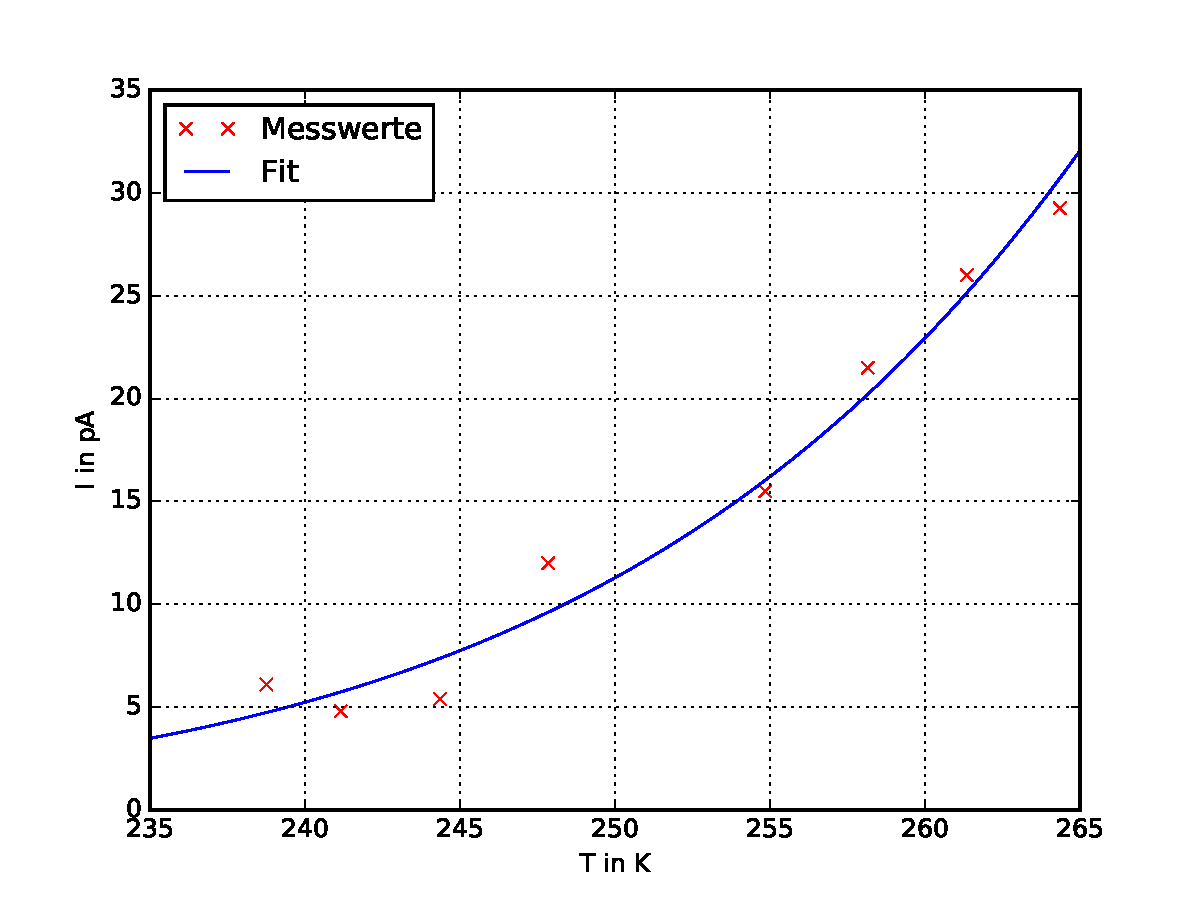
\includegraphics[width=0.8\textwidth]{plots/efit.pdf}
  \caption{Anlaufkurve des Depolarisationsstromes bei einer mittleren Heizrate von $H_1 =\SI{3.3 \pm 0.08}{\kelvin\per\minute}$.}
  \label{fig:efit1}
\end{figure}
\begin{figure}[H]
  \centering
  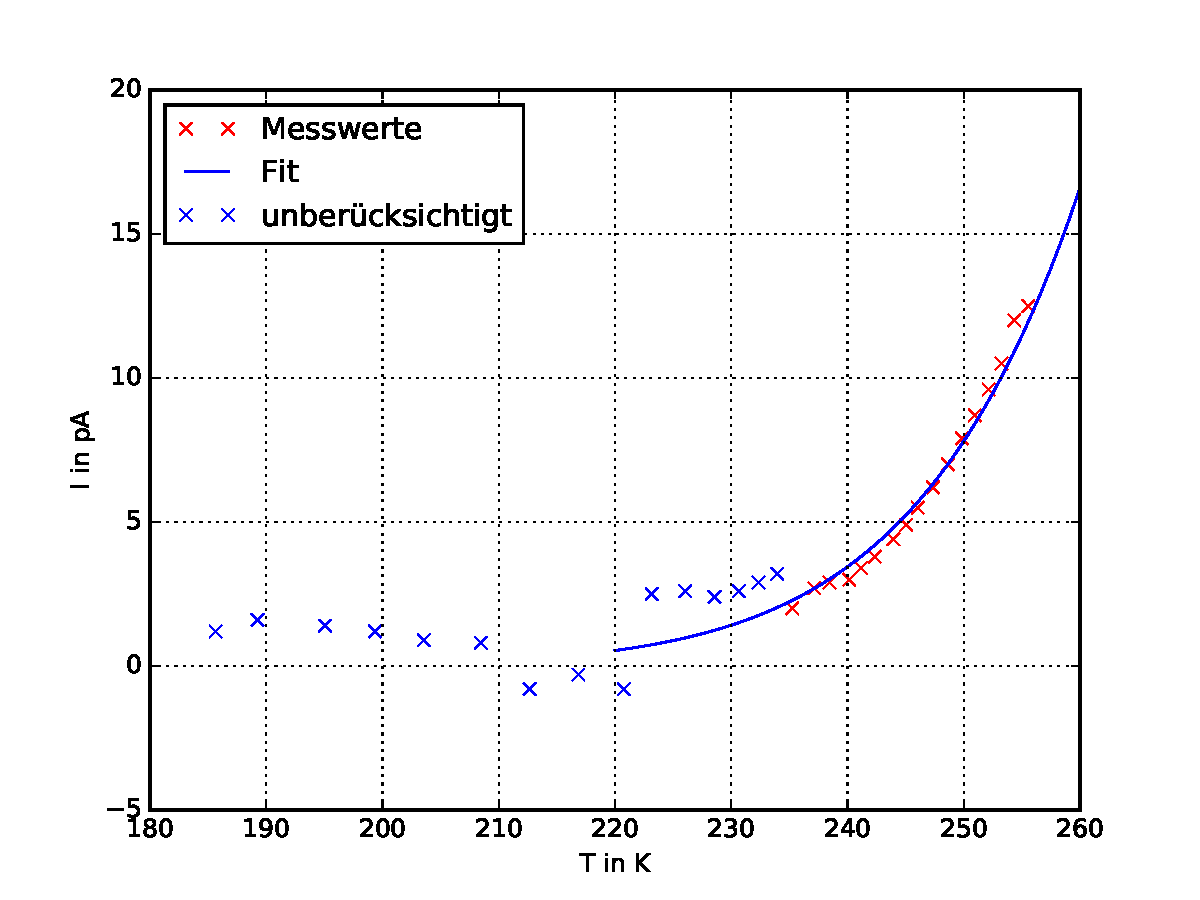
\includegraphics[width=0.8\textwidth]{plots/efit2.pdf}
  \caption{Anlaufkurve des Depolarisationsstromes bei einer mittleren Heizrate von $H_2 =\SI{1.26 \pm 0.07 }{\kelvin\per\minute}$}
  \label{fig:efit2}
\end{figure}
Die gefitteten Anlaufkurven sind in Abbildung \ref{fig:efit1} und \ref{fig:efit2} zu sehen.
Für den Fit der zweiten Messung wurden die in Abbildung \ref{fig:efit2} gezeigten bauen Messwerte nicht berücksichtigt.
Aus den angehängten Messwerten wurden ausserdem mittlere Heizraten für beide Messungen bestimmt. Die aus den Werten der Anlaufkurve ermittelten Heizraten lauten:
\begin{center}
  $H_1 =(3.2 \pm 0.13)\frac{\symup{K}}{\text{min}}$, $H_2 = (1.26 \pm 0.064)\frac{\symup{K}}{\text{min}}$
\end{center}
Aus der Ausgleichsrechnung ergeben sich die Fitparameter zu
\begin{center}
    $m_1 = 5680.23$, $ a_1= 24.98$, $m_2 = 5425.56$, $a_2 = 23.87$.
\end{center}
Aus dem Fitparameter $m_{(1/2)}$ werden dann nach
\begin{equation}
  W_{1/2} = m_{1/2}\cdot k_B
\end{equation}
die Austrittsarbeiten berechnet. Die berechneten Arbeiten lauten:
\begin{center}
  $W_1 = \SI{0.78e-19}{\joule}$ und $W_2 = \SI{0.75e-19}{\joule}$
\end{center}
